{\let\cleardoublepage\clearpage\chapter{Asperges}}

\section{Benedictio aquae}

\textit{%
    Die dominico, in sacristia praeparato sale et aqua benedicenda, sacerdos
    celebraturus Missam vel alius ad id deputatus, alba vel superpelliceo
    indutus cum stola circa collum, primo dicit:
}

\biblia{Ps. 123, 8}

\versiculum{Adiutorium nostrum in nomine Domini.}
{\setlength{\parskip}{0pt}
\par\responsorium{Qui fecit caelum et terram.}}

\textit{Deinde absolute incipit exorcismum salis.}

\initialis{E}xorcizo te, creatura salis, \ldots

\section{Aspersio aquae benedictae}

\vspace{-0.5\baselineskip}\directio{stans}

\textit{Extra tempus paschale sacerdos celebraturus, indutus pluviali coloris
officio convenientis, accedit ad altare, et ibi ad gradus cum ministris
genuflexus, etiam tempore paschali, accipit a diacono aspersorium, et primo ter
aspergit altare, deinde se, et erectus ministros, incipiens antiphonam} Asperges
me.  \textit{Et chorus prosequitur}: Domine, hyssopo, \textit{etc., ut infra.
Interim celebrans aspergit clerum, deinde populum.}

\vspace{0.5\baselineskip}
\begin{figure}[h]
    \centering
    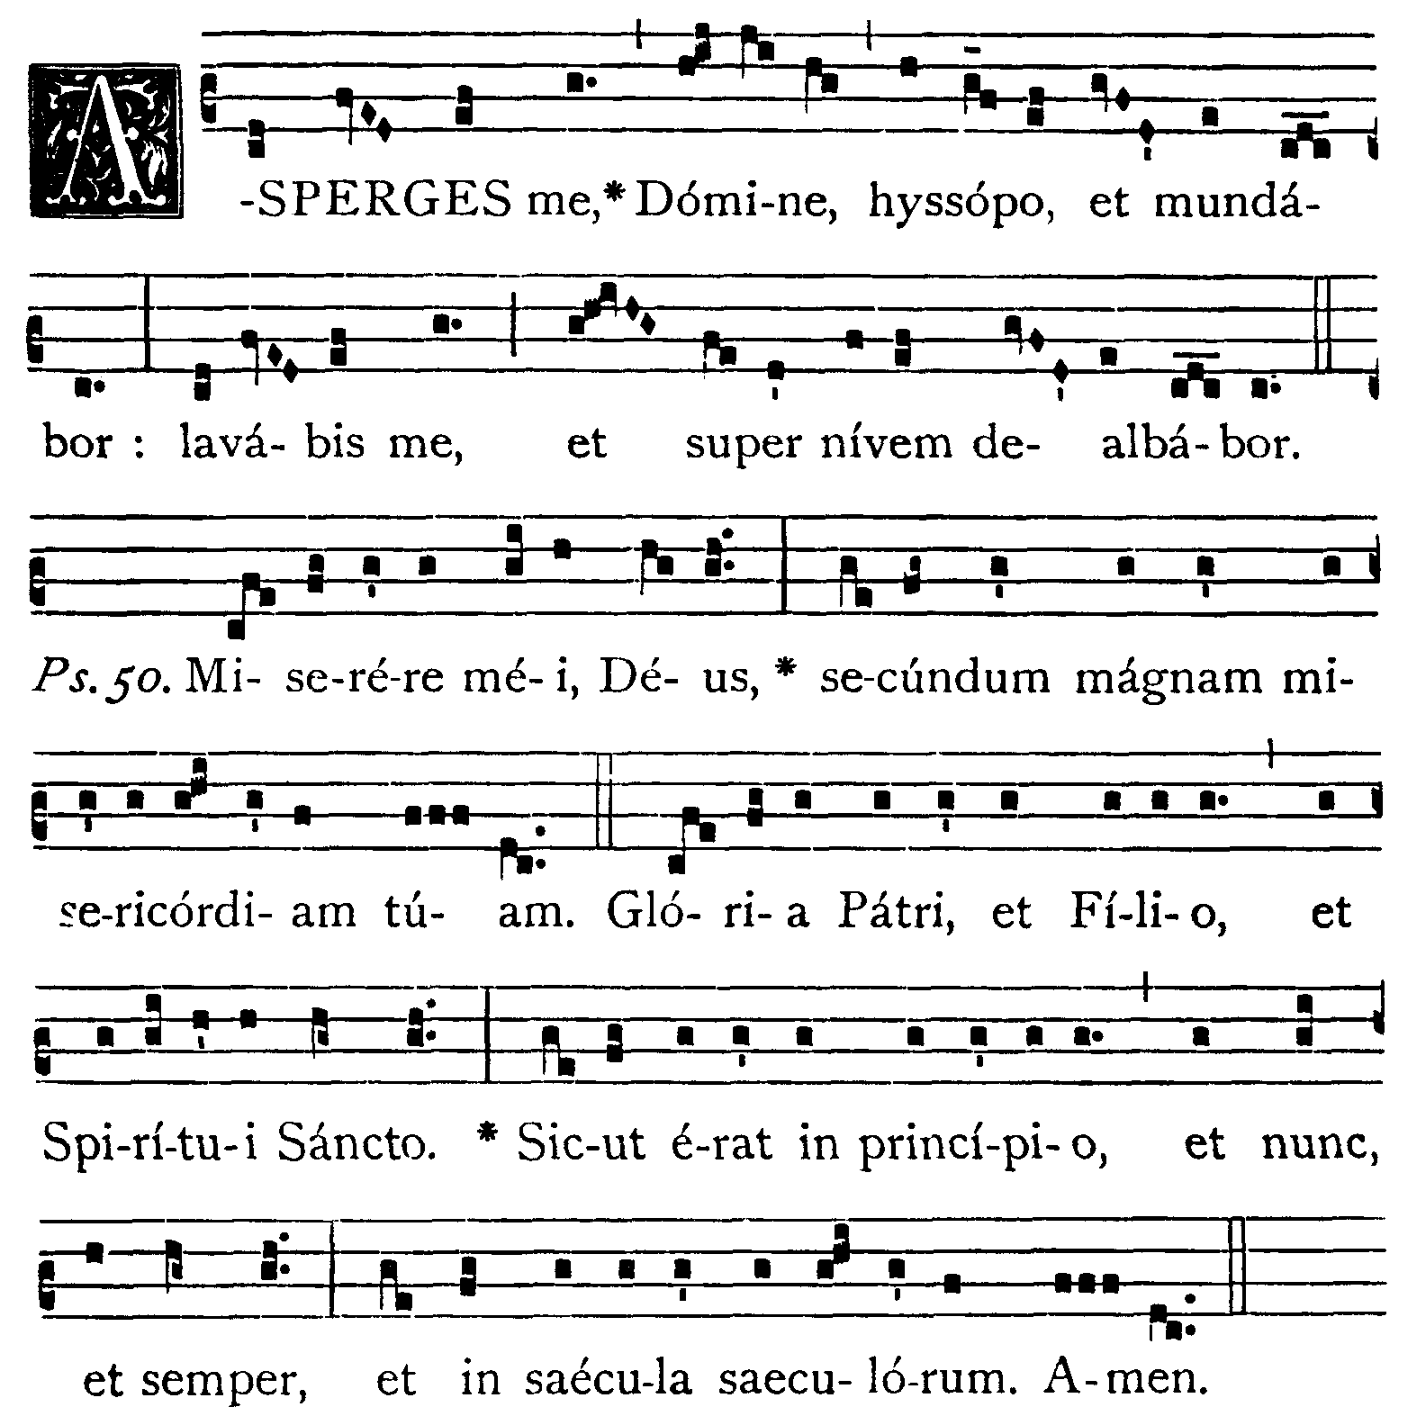
\includegraphics
        [scale=0.25, clip, viewport=1cm 42cm 30cm 49.5cm]
        {img/asperges.png}
\end{figure}
\vspace{0.5\baselineskip}

\begin{tabularx}{\dimexpr\textwidth-\parindent}{@{}p{5em}X@{}}
    \bibliafmt{Ps. 50, 9} &
    Asperges me (Domine) hyssopo et mundabor /
    lavabis me et super nivem dealbabor.
    \\ \noalign{\vspace{1em}}
    \bibliafmt{Ps. 50, 3} &
    Miserere mei, Deus, secundum magnam misericordiam tuam.
    \\ \noalign{\vspace{1em}}
    \bibliafmt{Doxologia \newline minor} &
    \directio{flectens} Gloria Patri, et Filio, et Spiritui Sancto: sicut erat
    in principio, et nunc, et semper, et in saecula saeculorum.  Amen.
    \\
\end{tabularx}

\divisio

\textit{%
    Tempore Passionis non dicitur Gloria Patris post psalmum Miserere, sed
    repetitur immediate antiphona Asperges Me.
}

\divisio

\directio{stans}

\textit{%
    Finita antiphona supradicto modo, sacerdos, qui aspersit aquam, reversus ad
    altare, stans ante gradus altaris, iunctis manibus, dicat:
}

\versiculum{Ostende nobis, Domine, misericordiam tuam.}
{\setlength{\parskip}{0pt}
\par\responsorium{Et salutare tuum da nobis.}
\par\versiculum{Domine, exaudi orationem meam.}
\par\responsorium{Et clamor meus ad te veniat.}
\par\versiculum{Dominus vobiscum.}
\par\responsorium{Et cum spiritu tuo,}}

Oremus.

\initialis{E}xaudi nos, Domine, sancte Pater, omnipotens aeterne Deus: et
mittere digneris sanctum Angelum tuum de caelis; qui custodiat, foveat,
protegat, visitet atque defendat omnes habitantes in hoc habitaculo.  Per
Christum Dominum nostrum.

\responsorium{Amen.}

\vfill
\begin{figure}[h]
    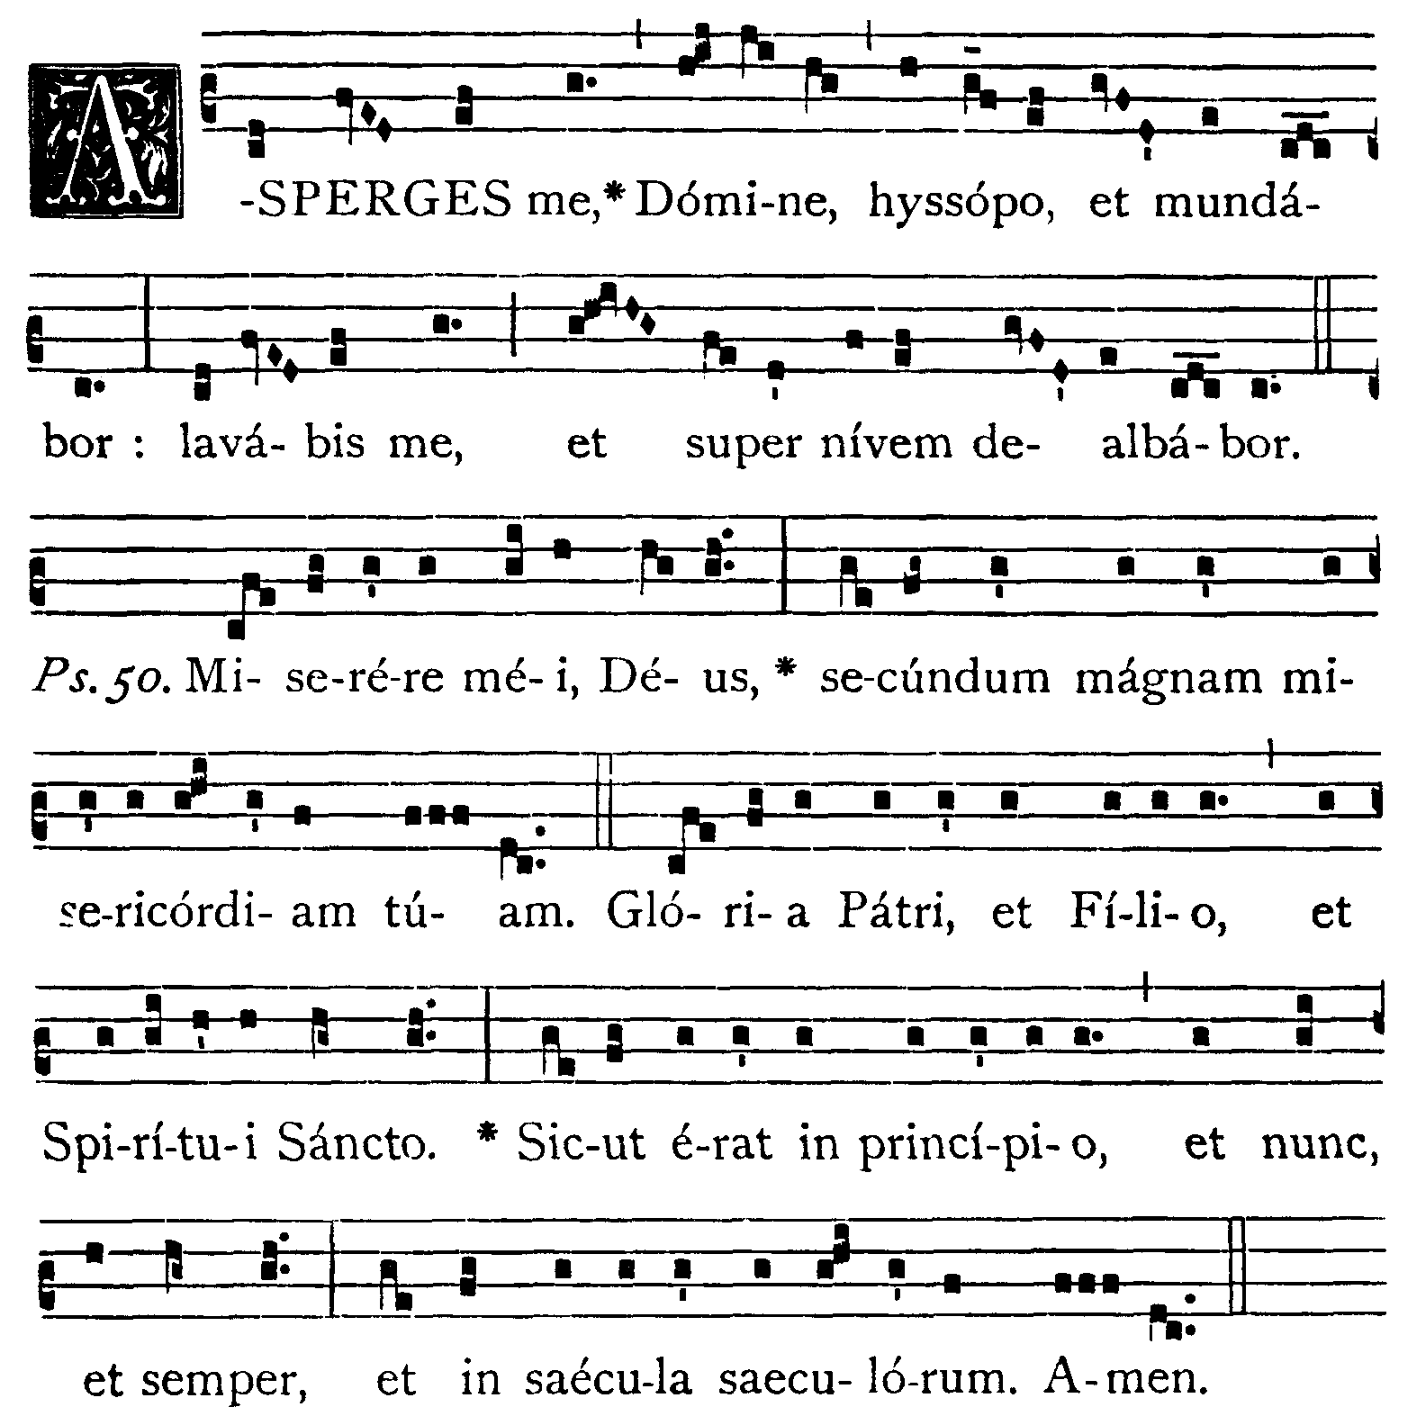
\includegraphics[width=\textwidth]{img/asperges.png}
\end{figure}
\vfill
